\documentclass{scrarticle}

\usepackage[english]{babel}    
\usepackage[T1]{fontenc}       
\usepackage[utf8]{inputenc} 
\usepackage{amsmath}           
\usepackage{amsfonts}          
\usepackage{amssymb}
\usepackage{graphicx} 
\usepackage{typearea}	        
\usepackage{scrlayer-scrpage}
\usepackage{lastpage}          
\usepackage{physics}
\usepackage{url}
\usepackage[margin=10pt,font=small,labelfont=bf]{caption}
\usepackage{subcaption}
\usepackage{comment}
\usepackage{url}
\usepackage{hyperref}
\usepackage{siunitx}
\usepackage{placeins}
\usepackage{verbatim}
\usepackage{cleveref}
\usepackage{braket}
\usepackage{dsfont}
\sisetup{separate-uncertainty, locale = UK}
\usepackage[backend=biber,sorting=none,style=numeric-comp]{biblatex}
\DeclareSIUnit\litre{l}

\addbibresource{ref.bib}

\title{Analytical timelike dssyk}
\author{georg}
\date{March 2026}

\begin{document}

\maketitle

\section{Find an analytical expression for $C_{ij;kl}$}

Generalized spacetime density kernal 
\begin{align}
    C_{ij; kl} = \text{Tr} \left[ \rho \ \hat{E}_{ij}^A \ U_t^\dagger \ \hat{E}_{kl}^B \ U_t \right]
\end{align}
with 
\begin{align}
    \hat{E}_{ij}^A = \ketbra{i}{j} \otimes  \mathds{1}_B \qquad \hat{E}_{kl}^B =  \mathds{1}_A \otimes \ketbra{k}{l}
\end{align}
For the DSSYK Tr[...] becomes just the expectation value $\bra{0}...\ket{0}$. For calculating the time evolution $U_t$ we also have to go into the continous energy basis $\ket{\theta}$. The energy basis features:
\begin{align}
    \mathds{1} = \int \frac{d\theta }{2 \pi} \mu(\theta) \ketbra{\theta}{\theta}
\end{align}
with 
\begin{align}
    \mu(\theta) = \left( q, e^{\pm 2 i\theta} \ ; q \right)_\infty.
\end{align}
This gives us 
\begin{align}
     C_{ij; kl} \propto \bra{0} \rho \ketbra{i}{j}  U_t^\dagger \ketbra{k}{l} U_t  \ket{0}
\end{align}
The overlaps with the chord basis 
\begin{align}
    \braket{\theta | n} = \frac{H_n(\cos(\theta)|q)}{\sqrt{(q; q)_\infty}}.
\end{align}
The energies in the eigenbasis are
\begin{align}
    E(\theta) = -\frac{2J \cos{\theta}}{\sqrt{\lambda(1-q)}}
\end{align}
We are stuck with integrals of the form
\begin{align}
    & \int_0^\pi \frac{d\theta}{2 \pi} \mu(\theta) \braket{\theta|n} e^{-i t E(\theta)} \\
    =& \int_0^\pi \frac{d\theta}{2 \pi} \left( q, e^{\pm 2 i\theta} \ ; q \right) \frac{H_n(\cos(\theta)|q)}{\sqrt{(q; q)_\infty}} e^{i t \frac{2J \cos{\theta}}{\sqrt{\lambda(1-q)}}}
\end{align}

\subsection{special case: SFF like Frobenius norm}
We can simplify the expression, if we calculate the $F_2$-norm from the kernal. The full kernal can be expressed as
\begin{align}
    C_{ij;kl}(t) = 
    \braket{0|\rho|i} \int \frac{d\theta d\phi}{(2\pi)^2} \ \mu(\theta) \mu(\phi) \
    e^{-i t(E(\theta)-E(\phi))} 
    \frac{H_j^*(\cos \theta |q) H_k(\cos \phi|q)}{\sqrt{(q;q)_j (q;q)_k}} \ 
    \frac{H_l^*(\cos\theta |q)}{\sqrt{(q;q)_l}}.
\end{align}
For the case of $\rho = \ketbra{0}{0}$ we can write calculate the frobenius norm
\begin{align}
    \sum_{i,j} C_{ij;ji}(t) = \sum_{i,j} \delta_{0i} &\int \frac{d\theta d\phi}{(2\pi)^2} \ \mu(\theta) \mu(\phi) \
    e^{-i t(E(\theta)-E(\phi))} 
    \frac{\left| H_j(\cos{\phi|q)} \right|^2}{(q;q)_j} \ 
    \frac{H_i^*(\cos\theta |q)}{\sqrt{(q;q)_i}},
\\
    &\int^\pi_0 \int^\pi_0 \frac{d\theta d\phi}{(2\pi)^2} \ \mu(\theta) \mu(\phi) \
    e^{-i t(E(\theta)-E(\phi))} 
    \label{eq:cijji}
\end{align}
\subsection{numerical evaluation of the SFF like Frobenius norm}
The sum over $C_{ij;ji}$ was calculated numerically involving numerical integration in Mathematica of integral \cref{eq:cijji}. The integrand is highly oscillating especially for large $t$ and also for high $q$ values.
\begin{figure}[htbp]
    \centering
    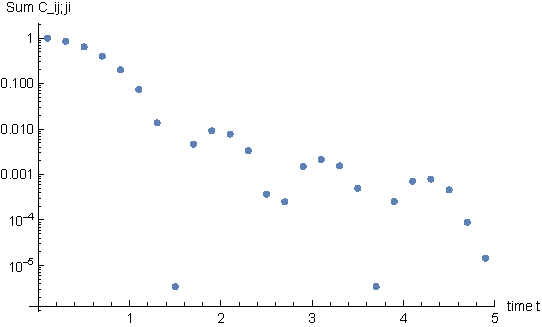
\includegraphics[width=0.5\linewidth]{plots/C_num.pdf}
    \caption{Numerical integration of expr. \cref{eq:cijji} for a value of $q = 0.1$}
    \label{fig:cijji_5}
\end{figure}
The computation (Mathematica) takes a long time due to higher oscillations for bigger $t$ and low $\lambda$, which is the regime we are interested in...
\begin{figure}[htbp]
    \centering
    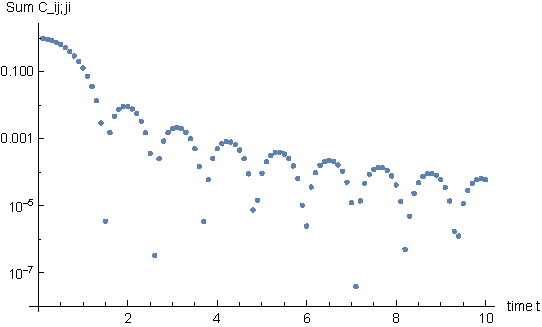
\includegraphics[width=0.5\linewidth]{plots/C_num2.pdf}
    \caption{Numerical integration of expr. \cref{eq:cijji} for a value of $q = 0.1$}
    \label{fig:cijji_50}
\end{figure}

\subsection{Calculating Two Time Correlators}
The purpose of defining a general response tensor $C_{ij;kl}$ is to easily compute two time correlators $\mathcal{L}_t(O_A, O_B)$ via the formula
\begin{align}
    \mathcal{L}_t(O_A, O_B) &= \text{Tr}\left[ \rho O_A U_t^\dagger O_B U_t \right] \nonumber \\
        &= \text{Tr}\left[T_{AB}(t) (O_A \otimes O_B) \right] \nonumber \\
        &= \sum_{i,j, k, l} C_{ij;kl} \ O_{ij}^{(A)} O_{kl}^{(B)}.
        \label{eq:two_time_c}
\end{align}
We briefly want to check that the kernel indeed does so by reproducing the two time correlator for the DSSYK given in \cite{berkooz_towards_2018} in eq. (3.16).\\
The observables in DSSYK are usually insertions of operators $M$ into our chord diagrams, which are simply fermion strings with random gaussian coefficients similar to the ones in our Hamiltonian. It is possible to compute the correlators via chord diagrams where each crossing of an $M$-string with an $H$-string is counted with a factor $\Tilde{q}$. In the analytic description one inserts a matrix 
\begin{align}
    S = \begin{pmatrix}
        1 & 0 & 0 & \ldots \\ 
        0 & \Tilde{q} & 0\\
        0 & 0&\Tilde{q}^2 \\
        \vdots & & & \ddots
    \end{pmatrix}.
\end{align}
So the operator coefficients we need are
\begin{align}
    O_{ij} = \delta_{ij} \ \Tilde{q}^j.
\end{align}
\\
We use $cos(\theta) = x$ and $cos(\phi) = y$. With this and $\rho = \ketbra{0}{0}$ equation \ref{eq:two_time_c} reads
\begin{align}
    \sum_{i,j, k, l} C_{ij;kl} \ O_{ij}^{(A)} O_{kl}^{(B)} = \sum_{i,j,k,l} \int &\frac{d\theta d\phi}{4 \pi^2} \mu(\theta) \mu(\phi) e^{i t(E(\theta) - E(\phi))} \cdot \nonumber
    \\ &\frac{H_j(x|q)}{\sqrt{(q;q)_j}} \frac{H_k(y|q) H_l(x|q)}{\sqrt{(q;q)_k}\sqrt{(q;q)_l}} \delta_{0i} \delta_{ij} \Tilde{q}^i \delta_{kl} \Tilde{q}^k
\end{align}
which simplifies to
\begin{align}
    \sum_{i,j, k, l} C_{ij;kl} \ O_{ij}^{(A)} O_{kl}^{(B)} 
    = \sum_{k} \int \frac{d\theta d\phi}{4 \pi^2} \mu(\theta) \mu(\phi) e^{i t(E(\theta) - E(\phi))} \frac{H_k(y|q) H_k(x|q)}{(q;q)_k} \Tilde{q}^k.
 \end{align}
Now we can use the identity for q-Hermite polynomials from \cite{berkooz_towards_2018} eq. (B.12) in the form \ref{eq:generating_funct} to get the desired form
\begin{align}
     \sum_{i,j, k, l} C_{ij;kl} \ O_{ij}^{(A)} O_{kl}^{(B)} =
     \int \frac{d\theta d\phi}{4 \pi^2} \mu(\theta) \mu(\phi) e^{i t(E(\theta) - E(\phi))} \frac{(\Tilde{q}^2, q)_\infty}{(\Tilde{q} e^{i(\pm \theta \pm \phi)}; q)_\infty},
\end{align}
which we can finde in \cite{berkooz_towards_2018} eq. (3.16) for euclidean time evolution.


\section{Doubled SYK model}
In the following, we want to calculate the coefficients $C_{ij;kl}$ of the spacetime density kernel $T_{AB}$ for the doubled SYK model of Narovlansky and Verlinde. We consider a bipartition of the system in the left and right SYK model. The starting point is, again, the formula
\begin{align}
    C_{ij; kl}(t) = \text{Tr} \left[ \rho \ \hat{E}_{ij}^L \ U_t^\dagger \ \hat{E}_{kl}^R \ U_t \right]
\end{align}
Here, $i$ and $j$ are chord numbers in the left subsystem, while $k$ and $l$ are chord numbers in the right subsystem. As shown by NV, the energy eigenstates of the system are given as paired eigenstates $\ket{E}=\ket{E}_L\ket{E}_R$. We insert two complete sets of energy eigenstates, labeled by $\theta$ and $\phi$, and obtain:
\begin{align}
    C_{ij;kl}(t) &= 
    \int \frac{d\theta d\phi}{(2\pi)^2} \ \mu(\theta) \mu(\phi) \braket{0|\rho \hat{E}_{ij}^L|\theta} \braket{\theta|U_t^\dagger\hat{E}_{kl}^RU_t|\phi}\braket{\phi|0}\\
    &= 
    \int \frac{d\theta d\phi}{(2\pi)^2} \ \mu(\theta) \mu(\phi) e^{-i t(E(\theta)-E(\phi))}\braket{0|\rho \hat{E}_{ij}^L|\theta} \braket{\theta|\hat{E}_{kl}^R|\phi}\braket{\phi|0}
\end{align}
The last scalar product simply yields 1. We evaluate the two matrix elements in this equation separately below. Firstly, we obtain, by setting $\rho=\ketbra{0}{0}$ for the density matrix:
\begin{align}
    \braket{0|\rho \hat{E}_{ij}^L|\theta}&=(\bra{0}\otimes\bra{0})(\ketbra{i}{j} \otimes  \mathds{1}_R)(\ket{\theta}\otimes\ket{\theta})\\
    &=\braket{0|i}\braket{j|\theta}\braket{0|\theta}.
\end{align}
Secondly, we obtain 
\begin{align}
    \braket{\theta|\hat{E}_{kl}^R|\phi}&=(\bra{\theta}\otimes\bra{\theta})( \mathds{1}_L\otimes \ketbra{k}{l})(\ket{\phi}\otimes\ket{\phi})\\
    &=\braket{\theta|\phi}\braket{\theta|k}\braket{l|\phi}.
\end{align}
Substituting back into eq. (15), we obtain:
\begin{align}
    C_{ij;kl}(t) &= \int \frac{d\theta d\phi}{(2\pi)^2} \ \mu(\theta) \mu(\phi) e^{-i t(E(\theta)+E(\phi))}\braket{0|i}\braket{j|\theta}\braket{0|\theta}\braket{\theta|\phi}\braket{\theta|k}\braket{l|\phi}\\
    &\propto\int \frac{d\theta d\phi}{(2\pi)^2} \ \mu(\theta) \mu(\phi) e^{-i t(E(\theta)+E(\phi))}\delta_{0i}\frac{H_j(\cos(\theta)|q)^*}{\sqrt{(q; q)_j}}\delta(\theta-\phi)\\
    &\quad\frac{H_k(\cos(\theta)|q)}{\sqrt{(q; q)_k}}\frac{H_l(\cos(\phi)|q)}{\sqrt{(q; q)_l}}\\
    &=\delta_{0i}\int \frac{d\theta}{2\pi}\mu(\theta)^2e^{-2i tE(\theta)}\frac{H_j(\cos(\theta)|q)^*}{\sqrt{(q; q)_j}}\frac{H_k(\cos(\theta)|q)}{\sqrt{(q;q)_k}} \frac{H_l(\cos(\theta)|q)}{\sqrt{(q; q)_l}}
\end{align}
We find that the result for $C_{ij;kl}(t)$ is given by a single integral. We would like to find a relation to the two-point function given by Verlinde:
\begin{equation}
    G_\Delta(\tau_1)=\braket{E_0|O_\Delta(\tau)O_\Delta(0)|E_0}=\int ds_1e^{-\tau_1E(s_1)}\frac{\Gamma_q(\Delta\pm is_0\pm is_1)\Gamma_q(1-\Delta\pm is_0\pm is_1)}{\Gamma_q(\pm 2is)\Gamma_q(2\Delta)\Gamma_q(2-2\Delta)}
\end{equation}
\section*{Appendix}

\begin{align}
    \sum_{k=0}^{\infty} H_k(x|q) H_k(y|q) \frac{t^k}{(q;q)_k} = \frac{(t^2, q)_\infty}{(t e^{i(\pm \theta \pm \phi)}; q)_\infty}
    \label{eq:generating_funct}
\end{align}

\newpage
\printbibliography

\end{document}